\documentclass[A4, 12pt]{article}

% Packages
	% Basics
		\usepackage{amsmath}
		\usepackage{amssymb}
		\usepackage{bm}
		\usepackage{csquotes}
		\usepackage[margin=0.75in]{geometry}
		\usepackage{hyperref}
		\usepackage[utf8]{inputenc}
	% Diagrams
		\usepackage{pgfplots}
		\usepackage{tikz}
	% Notation
		\usepackage{esint} % Integrals
		\usepackage{physics} 
		\usepackage{siunitx} % Units
	% Tables
		\usepackage{arydshln}
		\usepackage{multirow} 
% Configuration
	\title{Coulomb's Law Lab}
	\author{Arnav Patri}
	\hypersetup{
	    colorlinks,
	    citecolor=black,
	    filecolor=black,
	    linkcolor=black,
	    urlcolor=black
	}
% Macros
	% Utilities
		\newcommand{\callout}[2]{\begin{center}\fbox{\begin{minipage}{#1cm}#2\end{minipage}}\end{center}}
		\newcommand{\comment}[1]{}
		\newcommand{\subsectionb}[1]{\subsection*{#1}\addcontentsline{toc}{subsection}{#1}}
		\newcommand{\subsubsectionb}[1]{\subsubsection*{#1}\addcontentsline{toc}{subsubsection}{#1}}
		\newcommand{\subt}[2]{#1_{\text{#2}}}
\begin{document}
	\maketitle
	\begin{align*}
		\begin{array}{|*4{c|}}\hline
			\multicolumn{4}{|c|}{\textbf{Table 1}} \\\hline
			\multicolumn{2}{|c|}{q_1 = \SI{-4}{\micro C}} & \multicolumn{2}{|c|}{q_2 = \SI{8}{\micro C}} \\\hdashline
			r \,(\SI{}{cm}) & r^2 \,(\SI{}{m^2}) & 1/r^2 \,(\SI{}{m^{-2}}) & F_E \,(\SI{}{N}) \\\hline
			10 & 0.01 & 100 & 28.76\\
			9 & 0.0081 & \approx 123.457 & 35.506 \\
			8 & 0.0064 & 156.25 & 44.938 \\
			7 & 0.0049 & \approx 204.082 & 58.694 \\
			6 & 0.0036 & 277.\overline{7} & 78.889 \\
			5 & 0.0025 & 400 & 115.041 \\
			4 & 0.0016 & 625 & 179.751 \\
			3 & 0.0009 & 1111.\overline{1} & 319.557 \\\hline
		\end{array} &&
		\begin{array}{|*2{c|}}\hline
			\multicolumn{2}{|c|}{\textbf{Table 2}} \\\hline
			q_1 = \SI{5}{\micro C} & r = \SI{6}{cm} \\\hdashline
			q_2 (\SI{}{\micro C}) & F_E (\SI{}{N}) \\\hline
			10 & 124.827 \\
			9 & 112.344 \\
			8 & 99.862 \\
			7 & 87.379 \\
			6 & 74.896 \\
			5 & 62.414 \\
			4 & 49.931 \\
			3 & 36.448 \\\hline
		\end{array}
	\end{align*}
	\[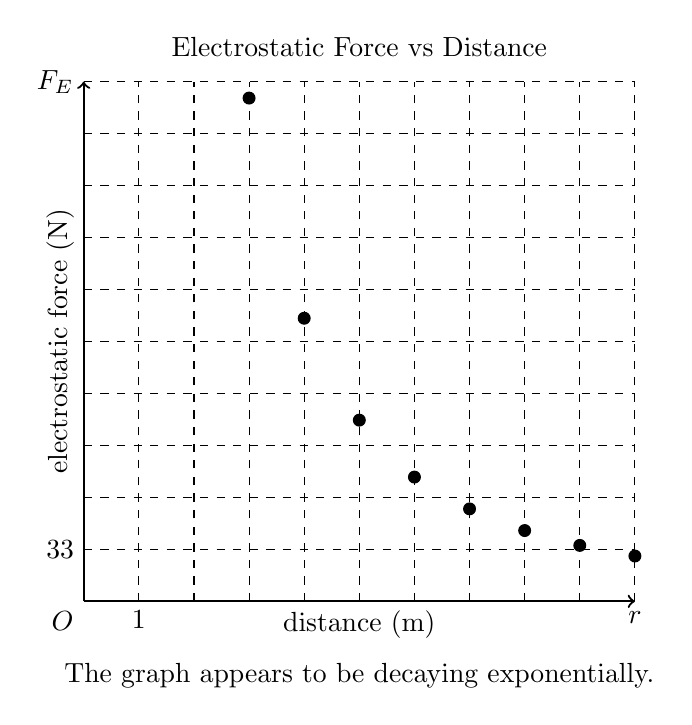
\begin{tikzpicture}[x = 7mm, y = 0.2mm]
		\node[above] at (5, 340) {Electrostatic Force vs Distance};
		\draw[thick, ->] (0, 0) node[anchor = north east]{\(O\)} -- (10, 0) node[below]{\(r\)};
			\node[below] at (5, 0) {distance (\SI{}{m})};
		\draw[thick, ->] (0, 0) -- (0, 330) node[left]{\(F_E\)};
			\node[rotate = 90, above] at (0, 165) {electrostatic force (\SI{}{N})};
		\foreach \x in {1,..., 10}
			\draw[dashed] (0, \x * 33) -- (10, \x * 33);
		\foreach \x in {1,..., 10}
			\draw[dashed] (\x, 0) -- (\x, 330);
		\node[below] at (1, 0) {1};
		\node[left] at (0, 33) {33};
		\foreach \x/\y in {10/28.76, 9/35.506, 8/44.938, 7/58.694, 6/78.889, 5/115.041, 4/179.751, 3/319.557}
			\filldraw (\x, \y) circle (0.75mm);
		\node[below] at (5, -33) {The graph appears to be decaying exponentially.};
		\end{tikzpicture}\]
	\[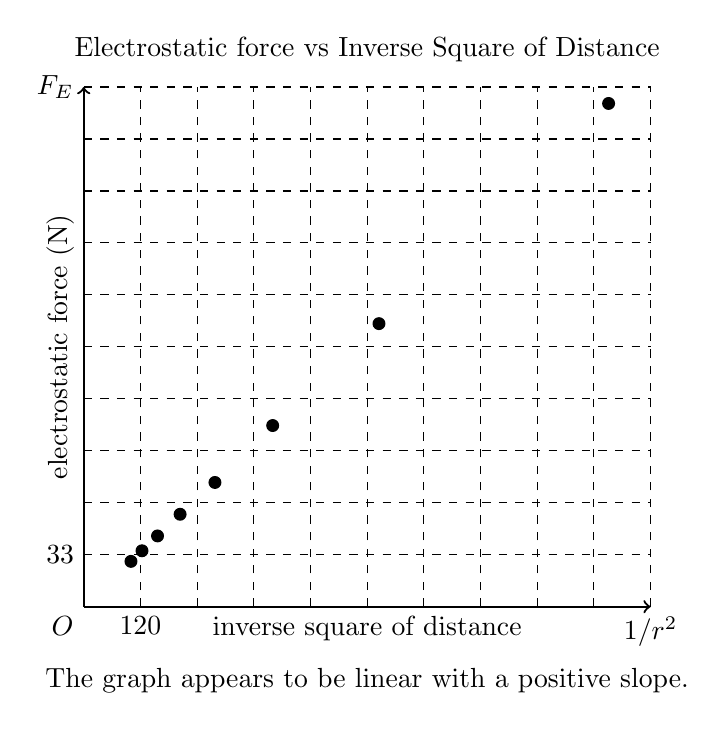
\begin{tikzpicture}[x = 0.06mm, y = 0.2mm]
		\node[above] at (600, 340) {Electrostatic force vs Inverse Square of Distance};
		\draw[thick, ->] (0, 0) node[anchor = north east]{\(O\)} -- (1200, 0) node[below]{\(1/r^2\)};
			\node[below] at (600, 0) {inverse square of distance};
		\draw[thick, ->] (0, 0) -- (0, 330) node[left]{\(F_E\)};
			\node[rotate = 90, above] at (0, 165) {electrostatic force (\SI{}{N})};
		\foreach \x in {1,..., 10}
			\draw[dashed] (0, \x * 33) -- (1200, \x * 33);
		\foreach \x in {1,..., 10}
			\draw[dashed] (\x * 120, 0) -- (\x * 120, 330);
		\node[below] at (120, 0) {120};
		\node[left] at (0, 33) {33};
		\foreach \x/\y in {100/28.78, 123.347/35.506, 156.25/44.938, 204.028/58.694, 277.78/78.889, 400/115.041, 625/179.751, 1111.1/319.557}
			\filldraw (\x, \y) circle (0.75mm);
		\node[below] at (600, -33) {The graph appears to be linear with a positive slope.};
	\end{tikzpicture}\]
	\[
		F_E = k\frac{|q_1||q_2|}{r^2} = 
				\frac{\text{slope}}{r^2} \approx 
			\implies k = \frac{\text{slope}}{|q_1||q_2|} 
				\approx \frac{0.2887}{|-4 \times 10^{-6}||8 \times 10^{-6}|} 
				\approx 9.022 \times 10^9
	\]
	\[\text{error} = \left|\frac{k - \subt{k}{known}}{\subt{k}{known}}\right| \approx 0.377 \%\]
	\[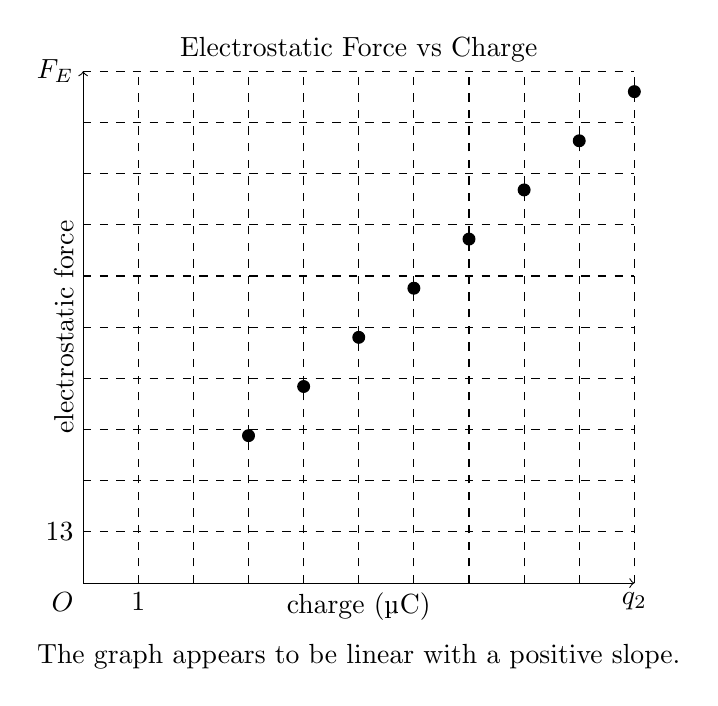
\begin{tikzpicture}[x = 7mm, y = 0.5mm]
		\node[above] at (5, 130) {Electrostatic Force vs Charge};
		\draw[->] (0, 0) node[anchor = north east]{\(O\)} -- (10, 0) node[below]{\(q_2\)};
			\node[below] at (5, 0) {charge (\SI{}{\micro C})};
		\draw[->] (0, 0) -- (0, 130) node[left]{\(F_E\)};
			\node[rotate = 90, above] at (0, 65) {electrostatic force};
		\foreach \x in {1,..., 10}
			\draw[dashed] (0, \x * 13) -- (10, \x * 13);
		\foreach \x in {1,..., 10}
			\draw[dashed] (\x, 0) -- (\x, 130);
		\node[below] at (1, 0) {1};
		\node[left] at (0, 13) {13};
		\foreach \x/\y in {10/124.827, 9/112.344, 8/99.862, 7/87.379, 6/74.896, 5/62.414, 4/49.931, 3/37.448}
			\filldraw (\x, \y) circle (0.75mm);
		\node[below] at (5, -13) {The graph appears to be linear with a positive slope.};
	\end{tikzpicture}\]
	\[
		F_E = k\frac{|q_1||q_2|}{r^2} 
				= \text{slope} \times 10^6 \times |q_2|
			\implies k = \frac{\text{slope} \times 10^6 \times r^2}{|q_1|} 
				\approx \frac{12.483 \times 10^6 \times 0.06^2}{|5 \times 10^{-6}|}
				\approx 8.988 \times 10^9
	\]
	\[\text{error} = \left|\frac{k - \subt{k}{known}}{\subt{k}{known}}\right| \approx 0.003 \%\]
\end{document}